%!TEX root = ../thesis.tex
In this chapter, we implement the discrete expressions for the expected total length of our one-dimensional model, as derived in Chapter 4.
First, we discuss how our Markov-modulated model can be used to recover various other models used throughout the literature through careful selection of the model parameters.
Where relevant, we also extend these models, or consider strategies that were not originally considered.
Finally, we investigate the most efficient search strategy according to our model, considering two-state and three-state Markov chains.

\section{Special cases of the Markov-modulated random walk strategy \label{sec:1dMMRW_specialcases}}
Our Markov-modulated random walk model can be seen as a more general version of many of the specific models that have been discussed in the literature.
To demonstrate this, we now demonstrate how careful selection of parameters in our model allows us to recover some of the more important models throughout the literature, or at the very least, high quality approximations to these models.

\subsection{Unmodulated random walk \label{sec:1dMMRW_nonMM}}

The random walk strategy with no Markov-modulation unsurprisingly exists as a special case of the Markov-modulated walk strategy, in which $Z$ has only a single state.
Consider the final expression found for the average total cost, \cref{eq:1dMMRW_cost:Q_neumann},
\begin{equation*}
\E{Q(a)} = \Tr{\left[ (\Id - {\Lmat})^{-1} \left( \vec{h}^\top\vec{z_0} \right) \right](a) } .
\end{equation*}

For the unmodulated case, we can consider an underlying Markov chain $Z$, which only has a single state ($J=1$), and hence $\vec{z_0}=[1]$, $r_v$ is constant, and the vector $\vec{h}(x)$ is the scalar function,
\begin{equation*}
h(x) = \mathbb{E}_{X_1\mid X_0}\left[q(X_0,X_1) \mid X_0 = x \right].
\end{equation*}

The operator $\Lmat$ now only consists of the element $\L_{1,1}$, which is
\begin{equation*}
[\L_{1,1} f] (x_n) = \int_{r_v}^{\lambda-r_v} p_1(x_n-x_{n-1})f(x_{n-1}) P_{1,1}(x_{n}) dx_{n-1},
\end{equation*}
which, after substituting in $P_{1,1}=1$, is equivalent to our operator $\L$ from the unmodulated section.
Substituting everything into \cref{eq:1dMMRW_cost:Q_neumann}, and leaving off the trace since this is a scalar, we arrive at
\begin{equation*}
\E{Q(a)} = \left[ (\Id - \L)^{-1} h  \right](a),
\end{equation*}
which matches with the expression found by Bartumeus \etal \cite{Bartumeus_2013}, and discussed in \cref{sec:1dRW}.

Using our Markov-modulated model, we set $P=[1]$, and $\vec{z_0} = [1]$ and investigate the efficiency over four different distributions: power-law, bounded power-law, exponential, and bounded exponential. We choose model parameters that match Bartumeus \etal \cite{Bartumeus_2013} to make comparisons easier. These are $\lambda=1000$, $ r_v=1$, and $\lmin = 1$. We also consider the effect of discretisation size on these results, plotting the efficiency for decreasing values of $\Delta x$, beginning with $\Delta x = 1$ and ending with $\Delta x = 0.2$, which was used by Bartumeus \etal \cite{Bartumeus_2013}.

\begin{figure}[h!]
	\centering
	\subfloat[{Destructive foraging ($x_0=\lambda/2$)}]{%
		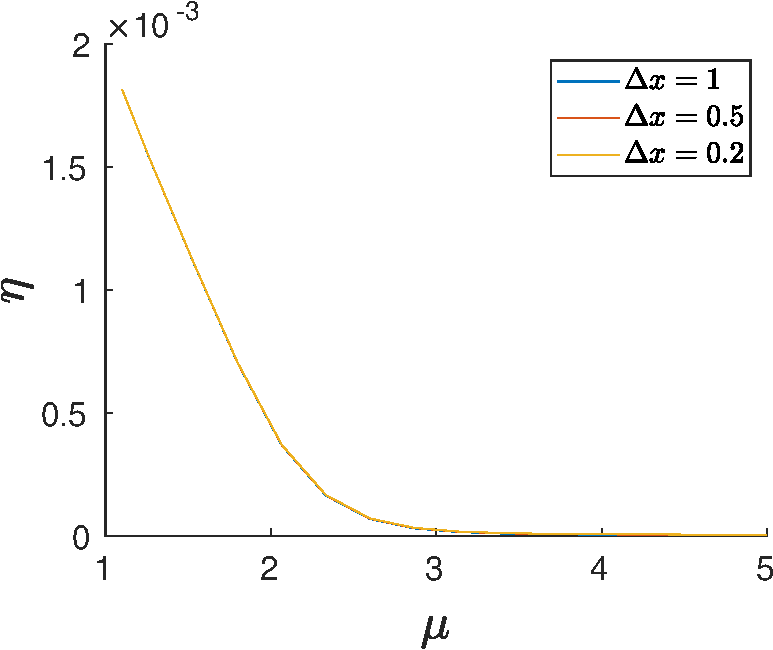
\includegraphics[width=.50\textwidth]{OneStateForager_varying-dx_PowerLaw_D_lambda1000_rv1_lmin1}\label{fig:OneStateForager_PowerLaw_D}}\hfill
	\subfloat[{Non-destructive foraging ($x_0=r_v$)}]{%
		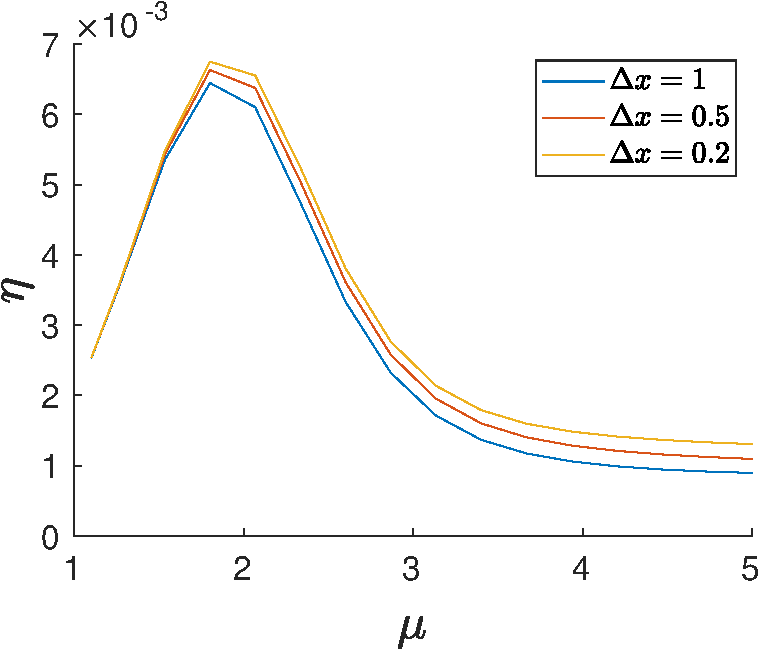
\includegraphics[width=.50\textwidth]{OneStateForager_varying-dx_PowerLaw_ND_lambda1000_rv1_lmin1}\label{fig:OneStateForager_PowerLaw_ND}}\\
	\caption[Search efficiency of an unbounded power-law strategy across a range of different discretisation sizes]{Search efficiency, $\eta$, versus distribution parameter $\mu$, of a power-law step-length distribution strategy with model parameters: $\lambda = 1000$, $r_v=1$, $\lmin = 1$, and simulations run with three different discretisation sizes, $\Delta x = \{1,0.5,0.2\}$. \label{fig:OneStateForager_PowerLaw}}
\end{figure}

\cref{fig:OneStateForager_PowerLaw_D,fig:OneStateForager_PowerLaw_ND} both match the results of Bartumeus \etal \cite{Bartumeus_2013} exactly. The optimal parameter, $\mu$, for destructive foraging with a power-law distribution is $\mu \to 1$, and for non-destructive foraging is $\mu \approx 2$, which matches the conclusions of the literature (e.g. \cite{Viswanathan_1999,Bartumeus_2013}). 

With the bounded power-law distribution, \cref{fig:OneStateForager_PowerLawBounded_D} shows that the efficiency appears to be very similar to the unbounded power-law, with the biggest difference coming as $\mu \to 1$. An explanation for this is that the closer $\mu$ to $1$, the more likely that there are steps that are large enough to be truncated. When $\mu$ is larger, especially $\mu \geq 3$, the distribution has a finite variance and the chances of taking a step larger than $\lmax = 100$ is very low. The non-destructive case is shown in \cref{fig:OneStateForager_PowerLawBounded_ND}, although the efficiency curve is approximately the same shape, there the peak efficiency is shifted slightly towards a larger $\mu$. The peak efficiency ($\eta \approx 3 \times 10^{-3}$) is also much lower than that of the unbounded power-law ($\eta \approx 7 \times 10^{-3}$). The most efficient choice of parameter is now slightly larger than $\mu = 2$, rather than slightly below $\mu = 2$ as with the unbounded distribution. The bounded power-law distribution for the non-destructive case also seems to be relatively sensitive to the discretisation size. 


\begin{figure}[h!]
	\centering
	\subfloat[{Destructive foraging ($x_0=\lambda/2$)}]{%
		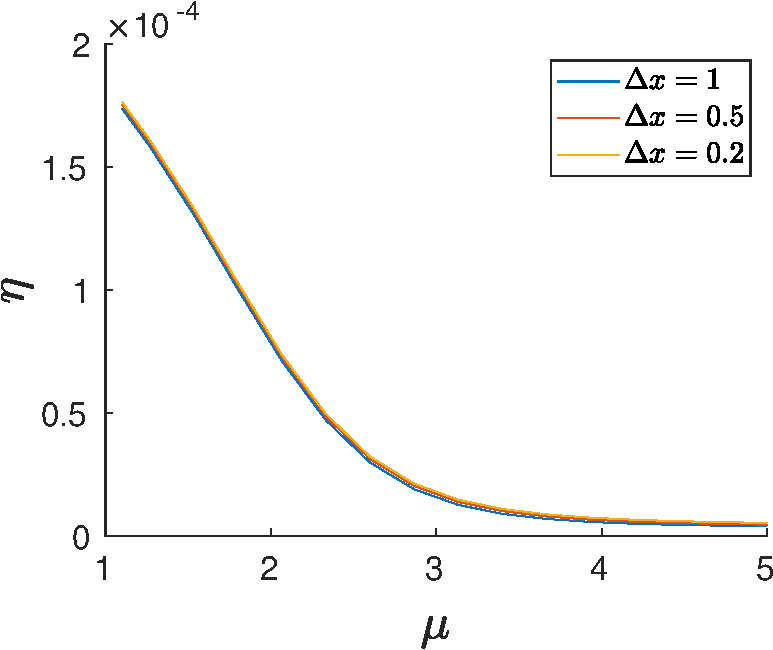
\includegraphics[width=.50\textwidth]{OneStateForager_varying-dx_PowerLawBounded_D_lambda1000_rv1_lmin1_lmax100}\label{fig:OneStateForager_PowerLawBounded_D}}\hfill
	\subfloat[{Non-destructive foraging ($x_0=r_v$)}]{%
		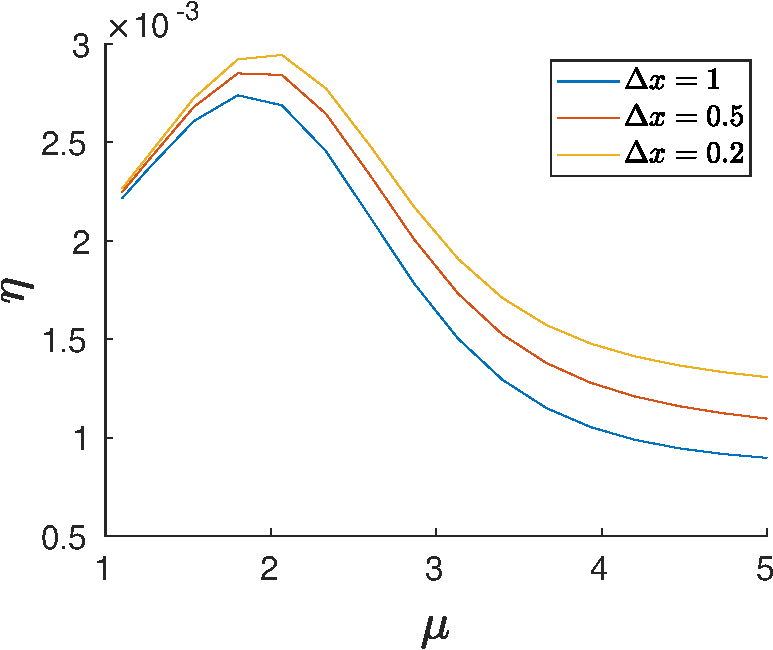
\includegraphics[width=.50\textwidth]{OneStateForager_varying-dx_PowerLawBounded_ND_lambda1000_rv1_lmin1_lmax100}\label{fig:OneStateForager_PowerLawBounded_ND}}\\
	\caption[Search efficiency of a bounded power-law strategy across a range of different discretisation sizes]{Search efficiency, $\eta$, versus distribution parameter $\mu$, of a bounded power-law step-length distribution strategy with model parameters: $\lambda = 1000$, $r_v=1$, $\lmin = 1$, $\lmax=100$, and simulations run with three different discretisation sizes, $\Delta x = \{1,0.5,0.2\}$ \label{fig:OneStateForager_PowerLawBounded}}
\end{figure}

To understand why the upper bound on the step-length distribution results in a worse efficiency, recall that for the unbounded power-law strategy, the peak efficiency was around $\mu=2$, which is a L\'{e}vy walk. This strategy would have mostly small steps, but every so often would take very large steps, allowing the forager to travel a large distance without any backtracking. However, with a small $\lmax$, the forager is unable to make these large steps,

The efficiency of the unbounded exponential strategy in \cref{fig:OneStateForager_Exponential_D} is optimal with $\mu \to 0$, and has a huge drop off immediately as $\mu$ increases. For the non-destructive search, the unbounded exponential has an optimal efficiency when $\mu \to 0$, as seen in \cref{fig:OneStateForager_Exponential_ND}. There is a large drop off in efficiency as $\mu$ increases, though not as extreme as in the destructive case. The efficiency in the non-destructive case seems to be relatively sensitive to discretisation size.


\begin{figure}[h!]
	\centering
	\subfloat[{Destructive foraging ($x_0=\lambda/2$)}]{%
		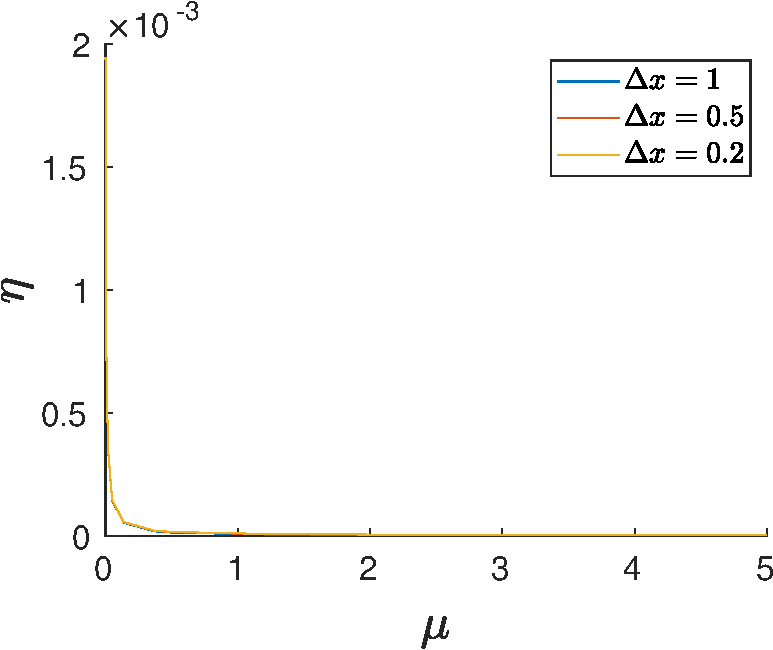
\includegraphics[width=.50\textwidth]{OneStateForager_varying-dx_Exponential_D_lambda1000_rv1_lmin1}\label{fig:OneStateForager_Exponential_D}}\hfill
	\subfloat[{Non-destructive foraging ($x_0=r_v$)}]{%
		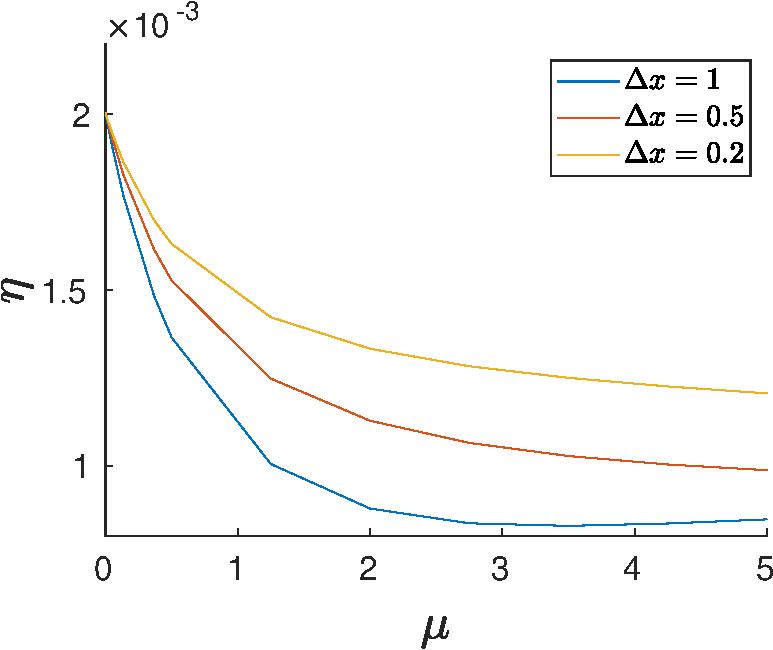
\includegraphics[width=.50\textwidth]{OneStateForager_varying-dx_Exponential_ND_lambda1000_rv1_lmin1}\label{fig:OneStateForager_Exponential_ND}}\\
	\caption[Search efficiency of an unbounded exponential strategy across a range of different discretisation sizes]{Search efficiency, $\eta$, versus distribution parameter $\mu$, of an exponential step-length distribution strategy with model parameters: $\lambda = 1000$, $r_v=1$, $\lmin = 1$, and simulations run with three different discretisation sizes, $\Delta x = \{1,0.5,0.2\}$. \label{fig:OneStateForager_Exponential}}
\end{figure}

Finally, we consider the bounded exponential in \cref{fig:OneStateForager_ExponentialBounded_D,fig:OneStateForager_ExponentialBounded_ND} for destructive and non-destructive foraging, respectively. The destructive foraging efficiency looks very similar to that of the unbounded exponential. The non-destructive foraging follows a similar pattern as the unbounded exponential distribution, although the drop off in efficiency as $\mu$ increases is not as pronounced. The optimal efficiency for both of these cases is found as $\mu \to 0$, which corresponds to the steps getting larger.


\begin{figure}[h!]
	\centering
	\subfloat[{Destructive foraging ($x_0=\lambda/2$)}]{%
		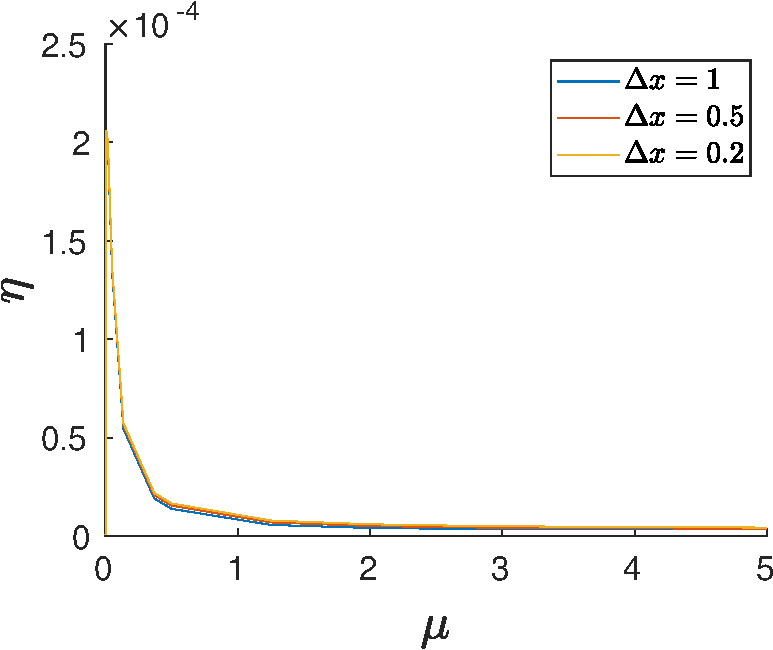
\includegraphics[width=.50\textwidth]{OneStateForager_varying-dx_ExponentialBounded_D_lambda1000_rv1_lmin1_lmax100}\label{fig:OneStateForager_ExponentialBounded_D}}\hfill
	\subfloat[{Non-destructive foraging ($x_0=r_v$)}]{%
		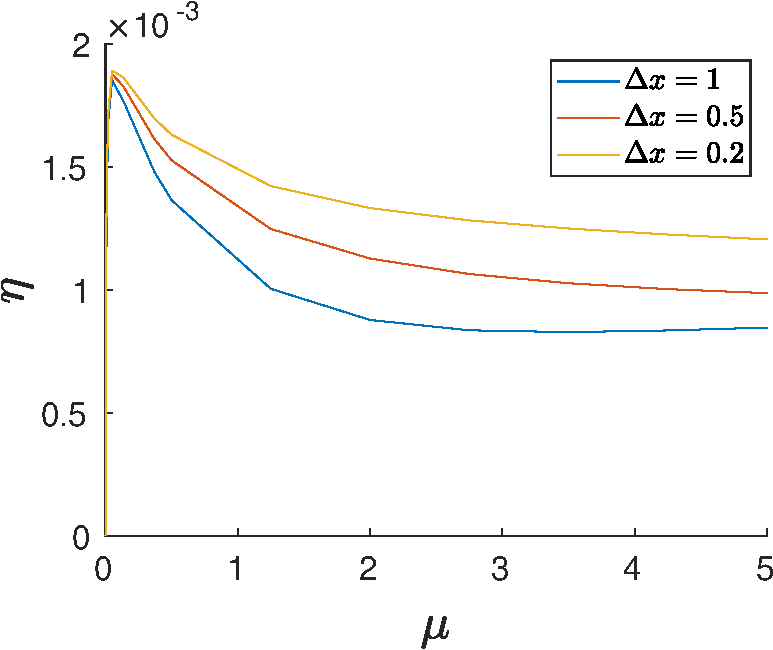
\includegraphics[width=.50\textwidth]{OneStateForager_varying-dx_ExponentialBounded_ND_lambda1000_rv1_lmin1_lmax100}\label{fig:OneStateForager_ExponentialBounded_ND}}\\
	\caption[Search efficiency of a bounded exponential strategy across a range of different discretisation sizes]{Search efficiency, $\eta$, versus distribution parameter $\mu$, of a bounded exponential step-length distribution strategy with model parameters: $\lambda = 1000$, $r_v=1$, $\lmin = 1$, $\lmax=100$, and simulations run with three different discretisation sizes, $\Delta x = \{1,0.5,0.2\}$ \label{fig:OneStateForager_ExponentialBounded}}
\end{figure}

It is worth noting that a strategy that involved simply choosing a direction at random and walking in a straight line (ballistic motion) will have an efficiency of $\eta = 2\times 10^{-3}$ for $\lambda = 10^{-3}$, since the expected distance travelled will be $\lambda/2$, regardless of starting position. Of the strategies investigated above, the only time an efficiency greater than $2 \times 10^{-3}$ was achieved was for both the bounded and unbounded power-law distributions, and only for non-destructive foraging. For the unbounded power-law distribution, if the parameter is in the approximate range $1.1 \leq \mu \leq 2.8$, then an efficiency greater than that of ballistic motion will be achieved. Similarly, for the bounded power-law distribution, although the range is slightly smaller, requiring approximately $1.1 \leq \mu \leq 2.6$.

To help summarise the results of comparing these four step-length distributions, we plot the efficiency of all four on a single plot, in \cref{fig:OneStateForager_AllDists_D} for destructive foraging and \cref{fig:OneStateForager_AllDists_ND} for non-destructive foraging. 


\begin{figure}[h!]
	\centering
	\subfloat[{Destructive foraging ($x_0=\lambda/2$)}]{%
		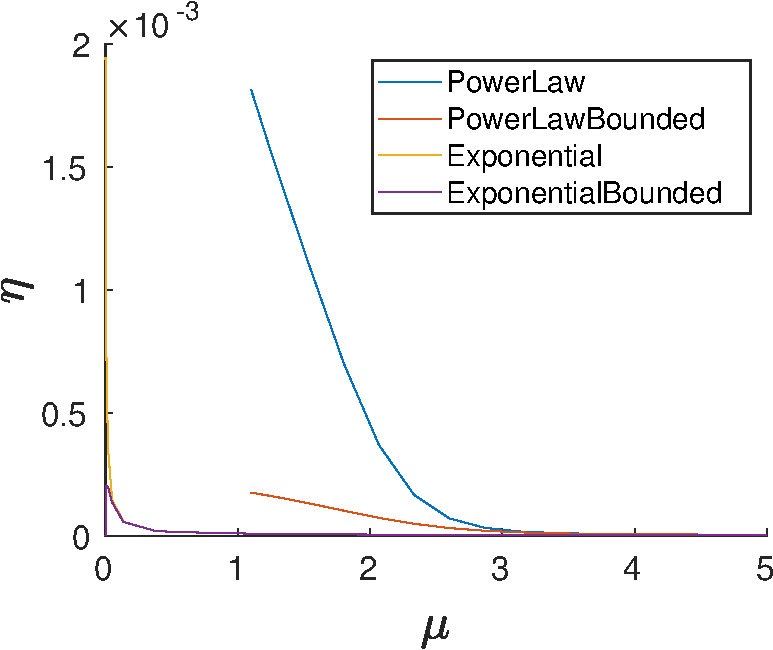
\includegraphics[width=.50\textwidth]{OneStateForager_AllDists_D_M5000_rv1_lmin1_lmax100}\label{fig:OneStateForager_AllDists_D}}\hfill
	\subfloat[{Non-destructive foraging ($x_0=r_v$)}]{%
		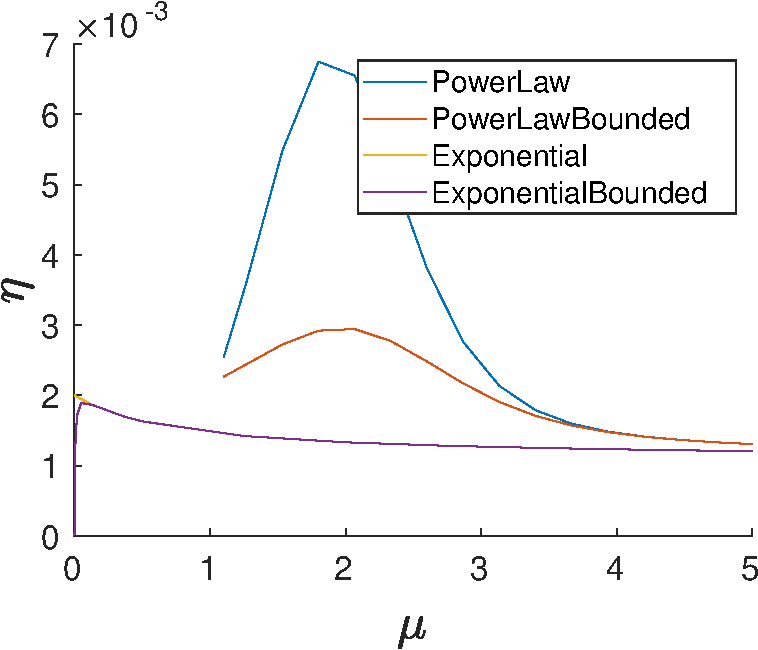
\includegraphics[width=.50\textwidth]{OneStateForager_AllDists_ND_M5000_rv1_lmin1_lmax100}\label{fig:OneStateForager_AllDists_ND}}\\
	\caption[Comparison of the search efficiency for the four different step-length distributions]{Search efficiency, $\eta$, versus distribution parameter $\mu$, for all four step-length distributions with model parameters: $\lambda = 1000$, $r_v=1$, $\lmin = 1$, $\lmax=100$, and simulations run using discretisation size $\Delta x =0.2$. \label{fig:OneStateForager_AllDists}}
\end{figure}

We also investigate the effect of the size of the upper bound, by plotting the efficiency of the bounded power-law and bounded exponential distributions for a range of $\lmax$, for both destructive and non-destructive foraging. Based on \cref{fig:EffectOfBound_PowerLawBounded_D,fig:EffectOfBound_PowerLawBounded_ND,fig:EffectOfBound_ExponentialBounded_D,fig:EffectOfBound_ExponentialBounded_ND}, the larger $\lmax$ is, the higher the efficiency of a foraging strategy, although for the exponential distribution an effect is only properly noticed for $\mu \to 0$. It is also worth noting that the graphs of the bounded distributions look the same as the corresponding unbounded distributions as $\lmax \to \infty$, which is to be expected since we recover the unbounded distributions as $\lmax \to \infty$. When $\lmax =1000$, the bounded distributions have a different distribution to the unbounded, even though a step can reach the boundary from any point, which seems counter-intuitive. This occurs because the bounded distribution is being normalised over $\lmin$ to $\lmax$, where $\lmax$ is finite, meaning larger steps are still less likely than they are for the unbounded distributions.

\begin{figure}[h!]
	\centering
	\subfloat[{Destructive foraging ($x_0=\lambda/2$)}]{%
		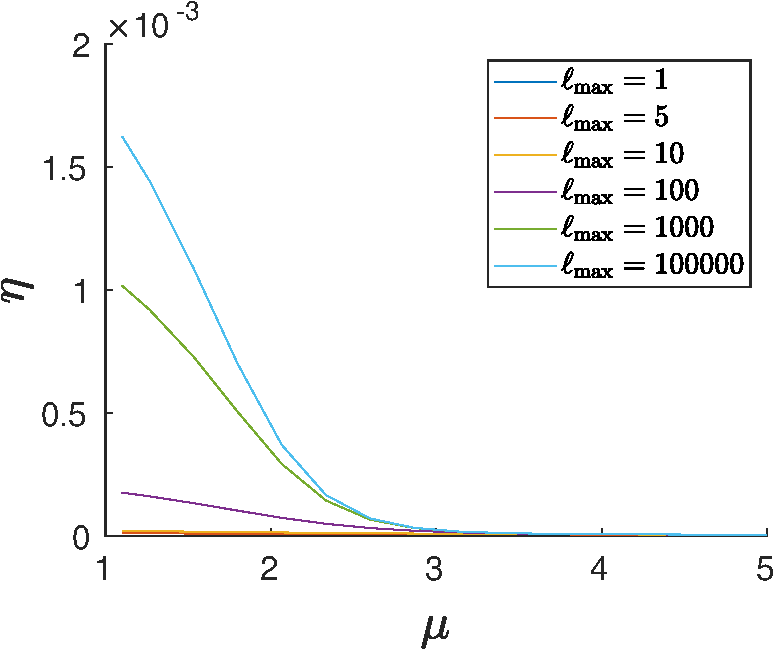
\includegraphics[width=.50\textwidth]{OneStateForager_varying-lmax_PowerLawBounded_D_M5000_rv1_lmin1}\label{fig:EffectOfBound_PowerLawBounded_D}}\hfill
	\subfloat[{Non-destructive foraging ($x_0=r_v$)}]{%
		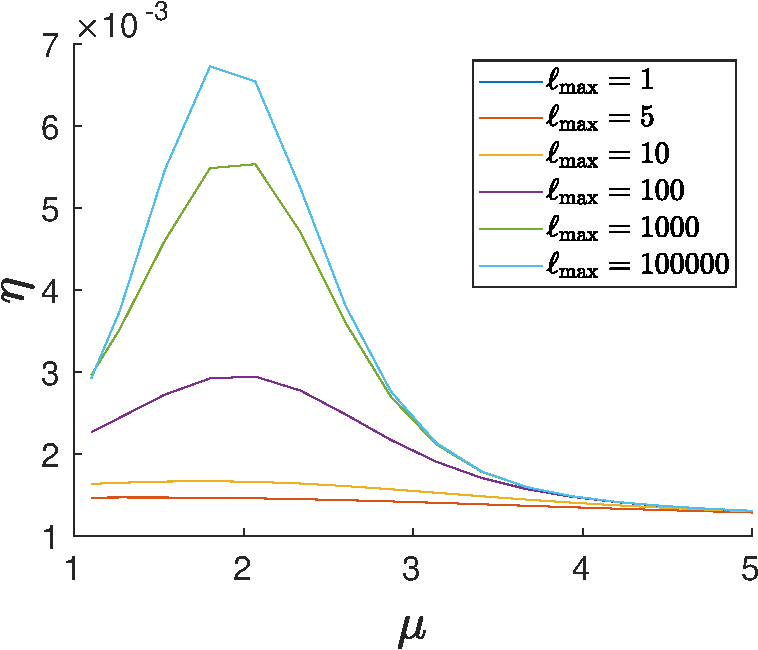
\includegraphics[width=.50\textwidth]{OneStateForager_varying-lmax_PowerLawBounded_ND_M5000_rv1_lmin1}\label{fig:EffectOfBound_PowerLawBounded_ND}}\\
	\caption[Effect of bound size on the search efficiency for a bounded power-law distribution for destructive foraging]{Search efficiency, $\eta$, versus distribution parameter $\mu$, for a bounded power-law distribution with model parameters: $\lambda = 1000$, $r_v=1$, $\lmin = 1$, $\Delta x=0.2$, and simulations run across multiple different upper bounds, $\lmax = \{1,5,10,100,1000\}$.\label{fig:EffectOfBound_PowerLawBounded}}
\end{figure}

\begin{figure}[h!]
	\centering
	\subfloat[{Destructive foraging ($x_0=\lambda/2$)}]{%
		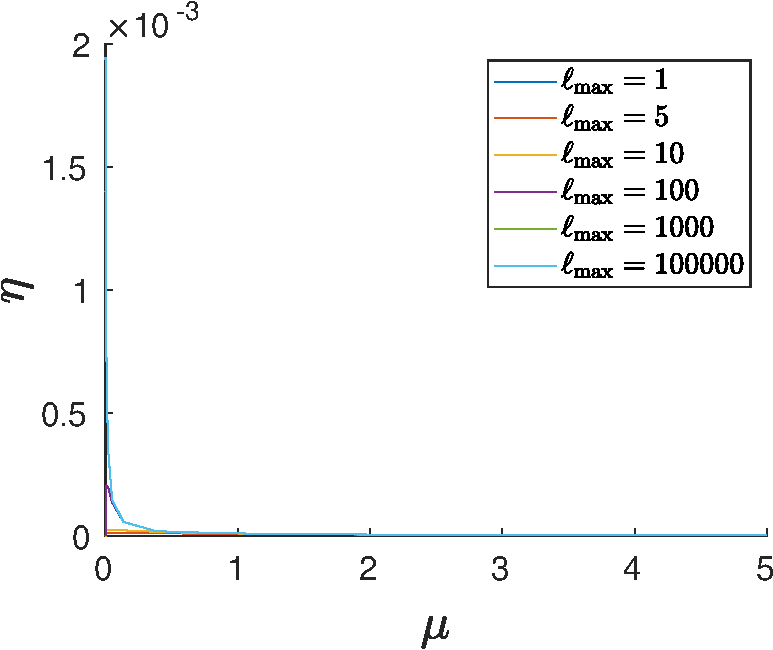
\includegraphics[width=.45\textwidth]{OneStateForager_varying-lmax_ExponentialBounded_D_M5000_rv1_lmin1}\label{fig:EffectOfBound_ExponentialBounded_D}}\hfill
	\subfloat[{Non-destructive foraging ($x_0=r_v$)}]{%
		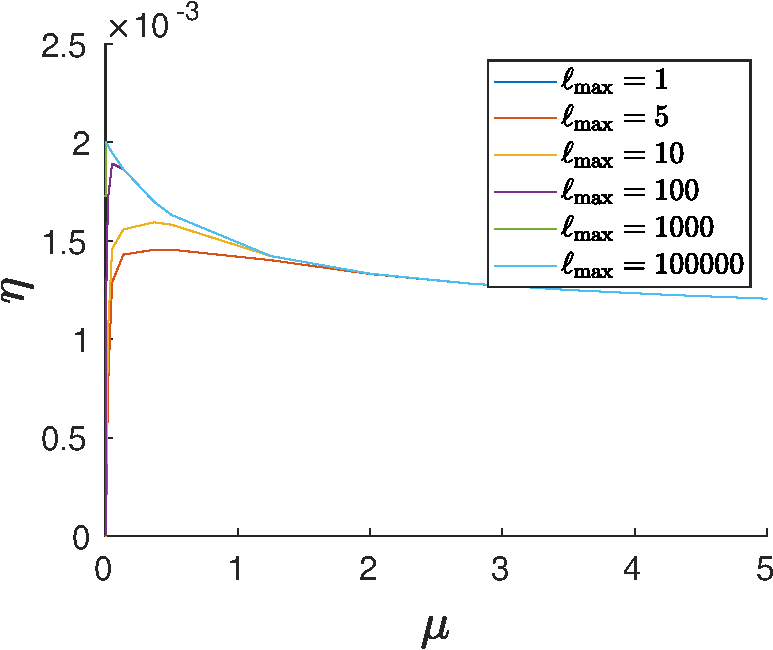
\includegraphics[width=.45\textwidth]{OneStateForager_varying-lmax_ExponentialBounded_ND_M5000_rv1_lmin1}\label{fig:EffectOfBound_ExponentialBounded_ND}}\\
	\caption[Effect of bound size on the search efficiency for a bounded exponential distribution for destructive foraging]{Search efficiency, $\eta$, versus distribution parameter $\mu$, for a bounded exponential distribution with model parameters: $\lambda = 1000$, $r_v=1$, $\lmin = 1$, $\Delta x=0.2$, and simulations run across multiple different upper bounds, $\lmax = \{1,5,10,100,1000\}$.\label{fig:EffectOfBound_ExponentialBounded}}
\end{figure}

\FloatBarrier
\subsection{Giving-up-time forager \label{sec:1dMMRW_GUT}}
Another special case of the Markov-modulated random walk is the random walk with ``giving-up time'', as discussed in papers by Benhamou \cite{Benhamou_2007}, Plank and James, \cite{Plank_2008}, and Reynolds \cite{Reynolds_2008_comment,Reynolds_2009_adaptive}.

These papers described a giving-up-time forager that undergoes an intensive search until some time, $\tau$, has elapsed, and then gives up its search and switches into an extensive search. The type of motion used in the intensive and extensive searches varies between papers, though most commonly it was Brownian motion and ballistic motion, respectively. Of the giving-up time strategies that have been investigated, the adaptive L\'{e}vy walk is the most general, which has Brownian motion for its intensive search, and the extensive search is drawn from a power-law distribution, where $\mu$ is allowed to take any value. Reynolds \cite{Reynolds_2009_adaptive} showed that his adaptive L\'{e}vy walk model could also model the previously investigated giving-up time models (e.g \cite{Plank_2008}) by setting $\mu \to 1$.

We now show that the adaptive L\'{e}vy walk can itself be thought of as a special case of a two-state Markov-modulated random walk. Furthermore, we have derived some analytic expressions for the efficiency in \cref{sec:1dMMRW_cost} and their discretised counterparts \cref{sec:1d_discrete:MMRW}, which should provide better accuracy compared to the results found by Reynolds \cite{Reynolds_2008_comment} via numerical simulation. We let state 1 represent the intensive search, and so \[p_1(x) = \frac{\mu_1-1}{\lmin}\left(\frac{\ell}{\lmin}\right)^{-\mu_1},\]
and state 2 represent the extensive search,
\[p_2(x) = \frac{\mu_2-1}{\lmin}\left(\frac{\ell}{\lmin}\right)^{-\mu_2}.\]

For a giving-up time model, the forager begins with an intensive search, and so $\vec{z_0} = (1,0)$.
When $\mu_1 \geq 3$, the intensive phase is a Brownian motion and hence we have the adaptive L\'{e}vy walk model of Reynolds \cite{Reynolds_2009_adaptive}. 
Further, when $\mu_1 \geq 3$ and $\mu_2 \to 1$, we recover the giving-up time strategy of Plank and James \cite{Plank_2008}. 
One of the earliest giving-up time strategies was the composite Brownian walk, which was introduced by Benhamou \cite{Benhamou_2007}. 
This involved exponentially distributed step-sizes for both the intensive and extensive search, though with different parameters for each. 
We may also model this using a two-state Markov-modulated random walk, by choosing exponential distributions for both states, although we do not do this since adaptive L\'{e}vy walks were found to have a better performance.

How we construct the transition matrix, $P$, will depend on how the giving-up-time, $\tau$, is defined.
For example, a geometrically distributed giving-up-time with expected value $1/p$ can be modelled with the transition matrix
\begin{equation}
\label{eq:P_geometricGUT}
P = \begin{bmatrix}
1-p & p\\
0 & 1
\end{bmatrix}.
\end{equation}
This geometric giving-up time will correspond to an exponential giving-up time in the continuous limit. If instead we have a deterministic giving-up-time, say $N$ steps before giving up, we can model this with the transition matrix
\begin{equation}
\label{eq:P_deterministicGUT}
P = \begin{bmatrix}
\vec{0}^T & \identity_N\\
0 & \vec{e}_N
\end{bmatrix},
\end{equation}
where $\vec{0} = (0,\dots,0)$ and $\vec{e}_N$ is a vector with the $N$th element a $1$ and all other elements are $0$. In this case, the first $N$ states of the Markov chain correspond to the same step-length distribution, $p_1(x)$, and the final state, state $N+1$, corresponds to the step-length distribution $p_2(x)$. 

By reordering the states of our Markov chain, we can write \cref{eq:P_geometricGUT,eq:P_deterministicGUT} in the form 
	\begin{equation*}
P = \begin{bmatrix}
1 & \vec{0} \\ 
\vec{t} & T
\end{bmatrix},
\end{equation*}
matching \cref{def:phase-type_dist}. That is, the giving-up time for both of these cases can be thought of as a discrete phase-type distribution. In fact, we can construct our states and transition matrix in such a way that we can consider any phase-type distribution for the giving-up time. Not only does this allow us to consider distributions such as geometric and negative-binomial, but using \cref{thm:PH-dense} we can approximate any possible distribution for the giving-up time using our Markov-modulated random walk.



\paragraph{Optimal giving-up time for Brownian motion giving up into ballistic motion}

Plank and James \cite{Plank_2008} described a forager that used a Brownian motion for its intensive search before giving-up into a ballistic motion for the extensive search. They were able to determine an approximate value for the optimal choice of giving-up time:
\begin{equation*}
\tau^* = \frac{d}{4v_I} \left( 1 - \frac{4}{3}\varepsilon -\frac{2}{5} \varepsilon^2 \right),
\end{equation*}
where $d$ is the distance between targets, $v_I$ is the velocity of the forager during the intensive search, and $\varepsilon = \frac{2x_0^2}{\pi v_I d} < 0.19$. If $\varepsilon > 0.19$ then the efficiency is optimised at $\tau = 0$, meaning the search is comprised entirely of ballistic motion. The average distance between patches, $d$, is equivalent to $\lambda$ in our model, and we are considering non-destructive foraging, which implies $x_0 = r_v$. Since we are considering the distance as opposed to the time required to find food, we have not yet discussed the velocity of a searcher. In the model of Plank and James \cite{Plank_2008}, a Brownian motion with variance $\sigma^2$ has velocity $v_I = \sqrt{2/\pi}\sigma$. Recalling \cref{ex:donskers}, the variance of a Brownian motion which arises as the limit of a random walk with unbounded power-law distributed steps is $\sigma^2 = (\mu-1)/(\mu-3) \lmin^2$, and we are choosing $\lmin=1$. Taking these differences into account, under our model we would expect the optimal giving-up time to be
\begin{equation*}
\tau^* = \frac{\lambda \sqrt{\pi}}{4 \sqrt{2} \sigma} \left( 1 - \frac{4}{3} \frac{2r_v^2}{\pi \lambda} - \frac{2}{5} \frac{4 r_v^4}{\pi^2 \lambda^2}\right),
\end{equation*}
with $\lambda \leq \frac{2 r_v^2}{0.19 \pi}$ implying that $\tau^* =0$. 

In our case, $\lambda = 1000$, $r_v=1$, and we choose $\mu =5$, so $\sigma = \sqrt{2}$ and $\lambda > \frac{2r_v^2}{0.19 \pi}$. Thus, the optimal giving-up time is 
\begin{equation*}
\tau^* = \frac{1000 \sqrt{\pi}}{8} \left( 1 - \frac{4}{3} \frac{2}{\pi 1000} - \frac{2}{5} \frac{4}{\pi^2 1000^2}\right) \approx 221.3686,
\end{equation*}
and so the optimal parameter $p = 1/\tau^* = 0.0045$.

We consider a Markov-modulated random walk with geometric giving-up time defined as above, with state $1$ being a power-law with $\mu =5 $, and state $2$ being a power-law with $\mu \to 1$. We use the transition matrix in \cref{eq:P_geometricGUT} and plot the efficiency of a non-destructive search for a range of different values of $p$ in \cref{fig:GeometricGUTForager_PowerLaw_ND_FixedMu}. We also use Matlab's \emph{fmincon} solver to find the optimal choice of $p$, and mark it on the plot. 

The optimal efficiency is $\eta =  0.0152$ and occurs at $p=0.0038$, which corresponds to a mean giving-up time of $263.4465$. This is not exactly the same as the value predicted by Plank and James \cite{Plank_2008}, but is a reasonable approximation, given the differences between their model and ours. Firstly, they considered a deterministic giving-up time, whereas we are considering a geometric giving-up time. We could consider a deterministic giving-up time, although to consider the values around this size, the matrix $\Amat$ would be far too large. Another difference between our model and theirs is that they considered continuous-time processes, whereas we are using discrete-time processes.

\begin{figure}[h!]
\centering
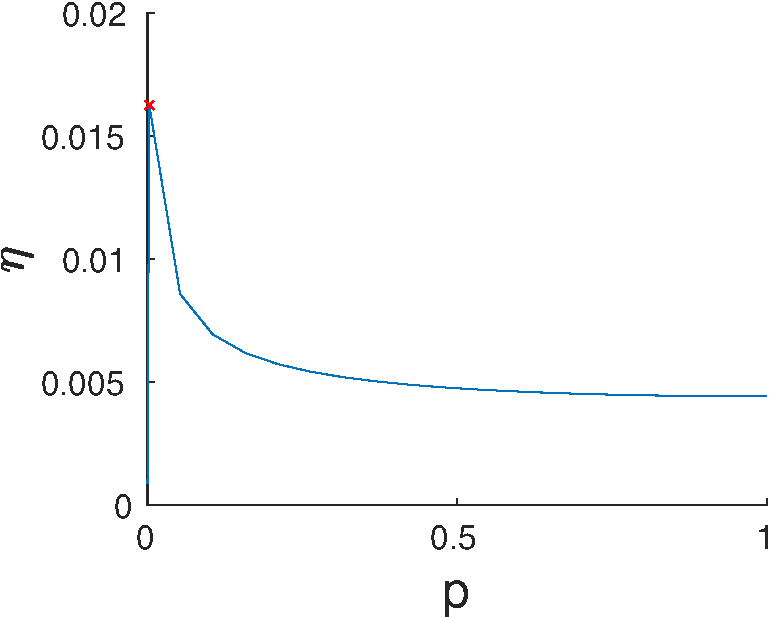
\includegraphics[scale=0.68]{GeometricGUTForager_PowerLaw_Fixedmu10-0-1-1_ND_lambda1000_rv1}
\caption[Efficiency vs geometric giving-up time parameter for a Brownian search that gives up and follows a ballistic path]{The efficiency of a non-destructive search ($x_0=r_v$) against the parameter $p$ for the geometric giving-up time. The forager uses a power-law distribution search with parameter $\mu_1 = 5$ before ``giving up'' and using a power-law search with $\mu_2 \to 1$. The peak efficiency (the red x) is $\eta = 0.0152$ which occurs at $p=0.0038$, corresponding to a mean giving-up time of $263.4465$. \label{fig:GeometricGUTForager_PowerLaw_ND_FixedMu}}
\end{figure}

\paragraph{Optimal adaptive L\'{e}vy walk parameters for fixed giving-up times}

As discussed in \cref{sec:litreview}, Reynolds \cite{Reynolds_2009_adaptive} investigated an adaptive L\'{e}vy walk, which involved switching between a power-law distribution with $\mu = 3$, and a power-law distribution with $\mu \to 1$, called the intensive and extensive phases, respectively. Reynolds also considered changing the values of $\mu$ during the extensive phase, and determined the optimal extensive search parameter. However, as correctly pointed out by Plank and James \cite{Plank_2008}, Reynolds only optimised over fixed giving-up times.

We now use our Markov-modulated random walk to investigate the adaptive L\'{e}vy walk model of Reynolds \cite{Reynolds_2009_adaptive}, although not only do we consider a range of different $\mu$ values for the extensive phase, but we also allow $\mu$ to vary in the intensive phase. We plot the efficiency at $40$ equispaced points in $1 < \mu_1 \leq 5$ and $1 < \mu_2 \leq 5$, for $5$ different choices of $p$ for a geometric giving-up time distribution.

The geometric giving-up time with the highest mean, $p=0.01$, had an optimal efficiency at $\mu_1 = 5$, and $\mu_2=1.6154$, as can be seen in \cref{fig:GeometricGUTForager_PowerLaw_ND_p0.01}. As the mean giving-up time was reduced, the optimal parameter for the intensive search does not change, but the extensive search parameter does change. For $p=0.1$ in \cref{fig:GeometricGUTForager_PowerLaw_ND_p0.1}, the optimal choice for the extensive parameter was $\mu_2= 1.7179$. For $p=0.5$, $p=0.9$, and $p=0.99$, in \cref{fig:GeometricGUTForager_PowerLaw_ND_p0.5,fig:GeometricGUTForager_PowerLaw_ND_p0.9,fig:GeometricGUTForager_PowerLaw_ND_p0.99} the optimal choice for the extensive parameter was $\mu_2=1.8205$. 

In all of these cases, the optimal extensive strategy is not a ballistic motion, but rather a L\'{e}vy flight, and the optimal intensive search is Brownian motion, matching the results of Reynolds \cite{Reynolds_2009_adaptive}. As the giving-up time increases, the extensive search gets closer to a ballistic motion, with a higher probability of very large steps, whereas for short giving-up times, the extensive parameter is closer to $\mu \approx 2$, which is the optimal for unmodulated search strategies.

In \cref{fig:GeometricGUTForager_PowerLaw_D_p0.01}, we also plot the efficiency of a giving-up time strategy for destructive foraging. Unsurprisingly, the optimal efficiency occurs at $\mu_1\to 1$ and $\mu_2 \to 1$, which is just a ballistic motion and not a true giving-up time strategy.

\begin{figure}[h!]
	\centering
	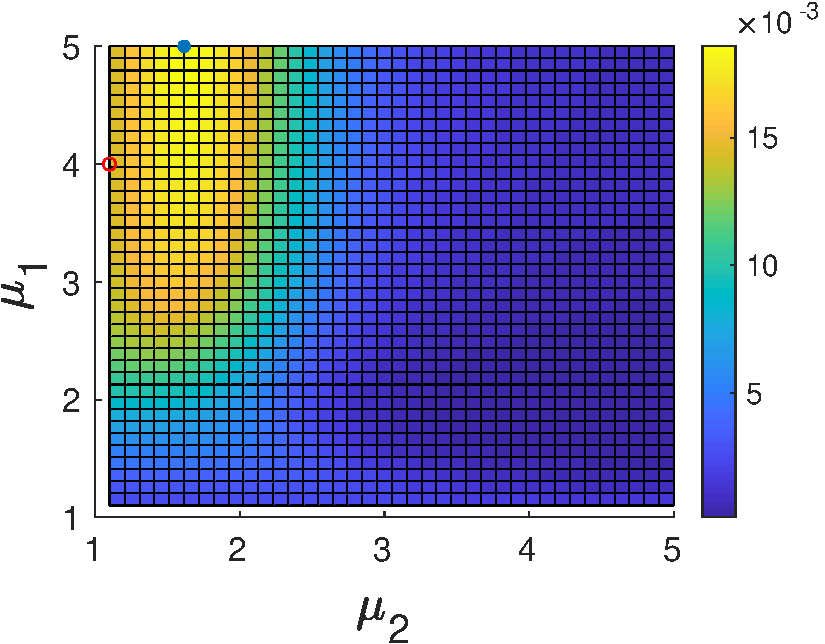
\includegraphics[scale=0.68]{GeometricGUTForager_FixedP0-01_PowerLaw_ND_lambda1000_rv1}
	\caption[Efficiency of two-state Markov-modulated power-law strategy, with giving-up parameter $p=0.01$, for non-destructive foraging]{The efficiency of a non-destructive search ($x_0=r_v$) where the forager uses a power-law distribution search with parameter $\mu_1$ before ``giving up'' and using a power-law search with $\mu_2$, after a geometrically distributed ($p=0.01$) amount of time has elapsed, which has a mean of $100$. The optimal efficiency is marked with the blue circle, and the red circle represents a Brownian motion giving-up into ballistic motion, although it is actually at any $\mu \geq 3$ rather than specifically at $\mu =4$.\label{fig:GeometricGUTForager_PowerLaw_ND_p0.01}}
\end{figure}

\begin{figure}[h!]
\centering
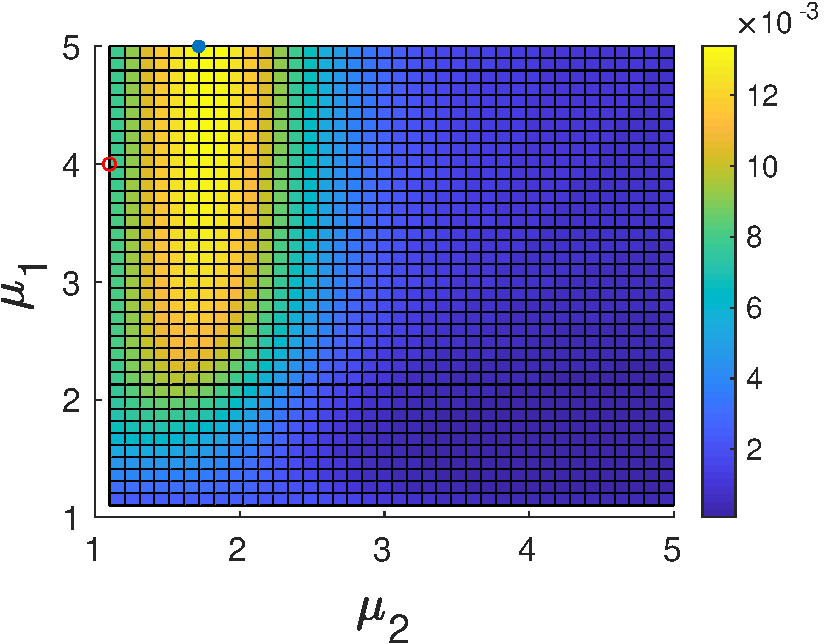
\includegraphics[scale=0.68]{GeometricGUTForager_FixedP0-10_PowerLaw_ND_lambda1000_rv1}
\caption[Efficiency of two-state Markov-modulated power-law strategy, with giving-up parameter $p=0.1$, for non-destructive foraging]{The efficiency of a non-destructive search ($x_0=r_v$) where the forager uses a power-law distribution search with parameter $\mu_1$ before ``giving up'' and using a power-law search with $\mu_2$, after a geometrically distributed ($p=0.1$) amount of time has elapsed, which has a mean of $10$. The optimal efficiency is marked with the blue circle, and the red circle represents a Brownian motion giving-up into ballistic motion, although it is actually at any $\mu \geq 3$ rather than specifically at $\mu =4$. \label{fig:GeometricGUTForager_PowerLaw_ND_p0.1}}
\end{figure}

\begin{figure}[h!]
	\centering
	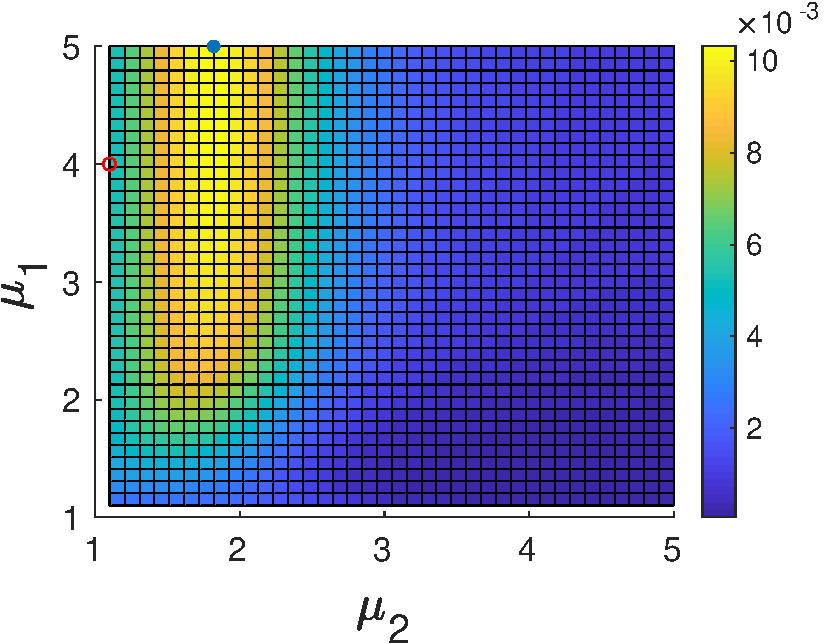
\includegraphics[scale=0.68]{GeometricGUTForager_FixedP0-50_PowerLaw_ND_lambda1000_rv1}
	\caption[Efficiency of two-state Markov-modulated power-law strategy, with giving-up parameter $p=0.5$, for non-destructive foraging]{The efficiency of a non-destructive search ($x_0=r_v$) where the forager uses a power-law distribution search with parameter $\mu_1$ before ``giving up'' and using a power-law search with $\mu_2$, after a geometrically distributed ($p=0.5$) amount of time has elapsed, which has a mean of $2$. The optimal efficiency is marked with the blue circle, and the red circle represents a Brownian motion giving-up into ballistic motion, although it is actually at any $\mu \geq 3$ rather than specifically at $\mu =4$. \label{fig:GeometricGUTForager_PowerLaw_ND_p0.5}}
\end{figure}

\begin{figure}[h!]
	\centering
	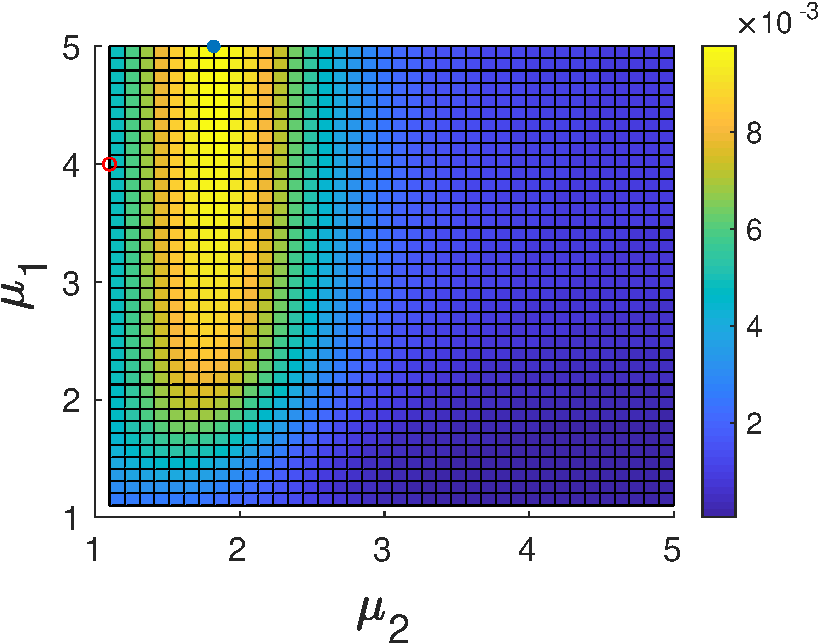
\includegraphics[scale=0.68]{GeometricGUTForager_FixedP0-90_PowerLaw_ND_lambda1000_rv1}
	\caption[Efficiency of two-state Markov-modulated power-law strategy, with giving-up parameter $p=0.9$, for non-destructive foraging]{The efficiency of a non-destructive search ($x_0=r_v$) where the forager uses a power-law distribution search with parameter $\mu_1$ before ``giving up'' and using a power-law search with $\mu_2$, after a geometrically distributed ($p=0.9$) amount of time has elapsed, which has a mean of approximately $1.11$. The optimal efficiency is marked with the blue circle, and the red circle represents a Brownian motion giving-up into ballistic motion, although it is actually at any $\mu \geq 3$ rather than specifically at $\mu =4$. \label{fig:GeometricGUTForager_PowerLaw_ND_p0.9}}
\end{figure}

\begin{figure}[h!]
	\centering
	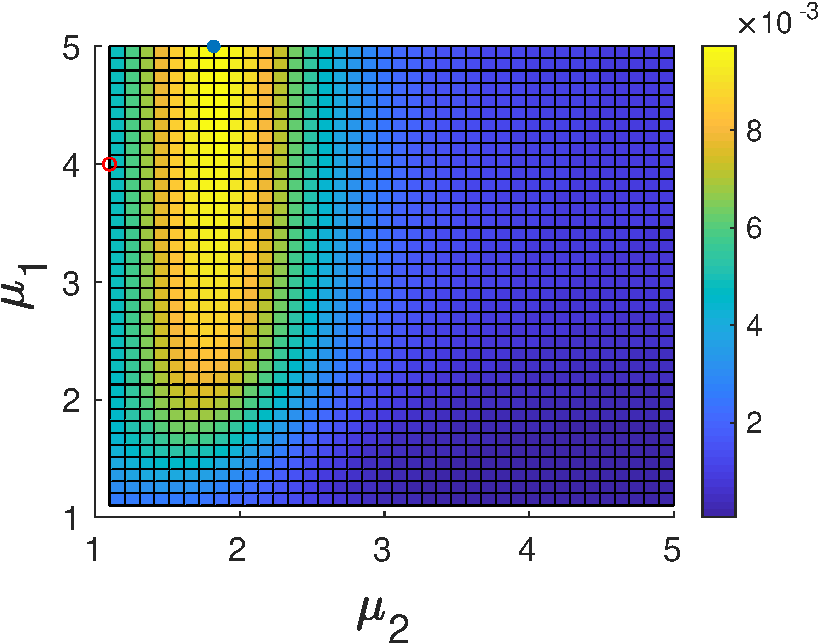
\includegraphics[scale=0.68]{GeometricGUTForager_FixedP0-99_PowerLaw_ND_lambda1000_rv1}
	\caption[Efficiency of two-state Markov-modulated power-law strategy, with giving-up parameter $p=0.99$, for non-destructive foraging]{The efficiency of a non-destructive search ($x_0=r_v$) where the forager uses a power-law distribution search with parameter $\mu_1$ before ``giving up'' and using a power-law search with $\mu_2$, after a geometrically distributed ($p=0.99$) amount of time has elapsed, which has a mean of $1.010101$. The optimal efficiency is marked with the blue circle, and the red circle represents a Brownian motion giving-up into ballistic motion, although it is actually at any $\mu \geq 3$ rather than specifically at $\mu =4$. \label{fig:GeometricGUTForager_PowerLaw_ND_p0.99}}
\end{figure}

\begin{figure}[h!]
	\centering
	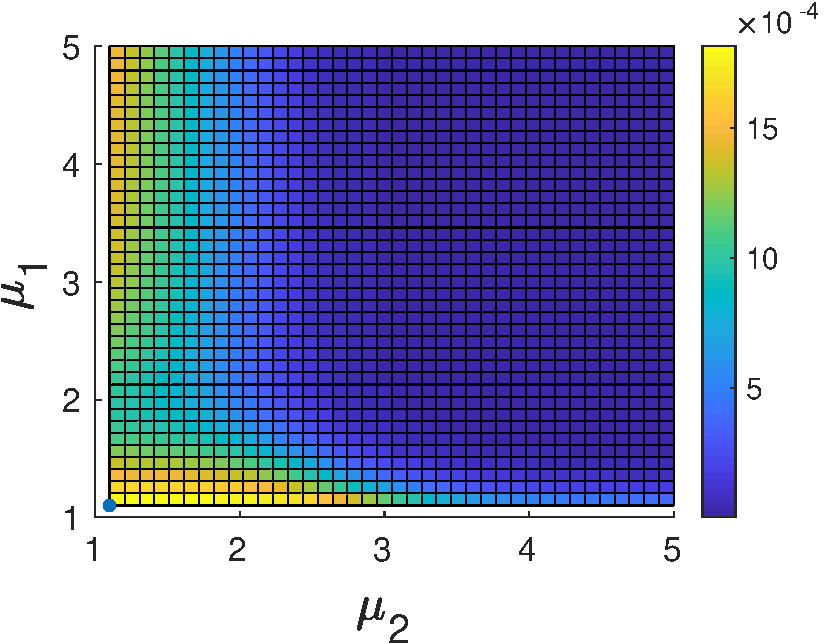
\includegraphics[scale=0.68]{GeometricGUTForager_FixedP0-01_PowerLaw_D_lambda1000_rv1}
	\caption[Efficiency of two-state Markov-modulated power-law strategy, with giving-up parameter $p=0.01$, for destructive foraging]{The efficiency of a destructive search ($x_0=\lambda/2$) where the forager uses a power-law distribution search with parameter $\mu_1$ before ``giving up'' and using a power-law search with $\mu_2$, after a geometrically distributed ($p=0.01$) amount of time has elapsed, which has a mean of $100$. The optimal efficiency is marked with the blue circle.\label{fig:GeometricGUTForager_PowerLaw_D_p0.01}}
\end{figure}

\FloatBarrier

\paragraph{Optimal geometric giving-up time strategy}

In the previous two parts, we considered the giving-up time models of Plank and James \cite{Plank_2008} and Reynolds \cite{Reynolds_2009_adaptive}. However, both of these have advantages and disadvantages. Plank and James \cite{Plank_2008} were able to find the optimal giving-up time, but considered only Brownian motion giving-up into ballistic motion. On the other hand, Reynolds \cite{Reynolds_2009_adaptive} found the optimal extensive parameters, but considered only fixed giving-up times. As shown above, we were able to use our Markov-modulated random walk strategy to investigate both of these models. Now, we can combine these ideas and use our model to optimise over both the giving-up time and the parameters $\mu_1$ and $\mu_2$.

We make use of Matlab's \emph{fmincon} function to minimise the expected total travel length, and hence maximise the efficiency over the three different parameters. We use the constraints that $0 \leq p \leq 1$, $1 < \mu_1 \leq 10$ and $1 < \mu_2 \leq 10$. 

For a non-destructive search, \emph{fmincon} finds the optimal efficiency at $p=0.0060$, $\mu_1 = 10.0000$, and $\mu_2 = 1.5868$. This value of $p$ corresponds to a mean giving-up time of approximately $167$, and the optimal values of $\mu$ correspond to a Brownian motion for the intensive search that gives up into a L\'{e}vy walk for the extensive search. The optimal value of $\mu_1 = 10$ was the maximum allowed value of $\mu_1$ according to our constraints. Increasing this upper bound will change the optimal value of $\mu_1$ accordingly, although it only changes the efficiency very slightly.

\subsection{Vision switching forager \label{sec:1dMMRW_VisionSwitching}}
Benichou \etal \cite{Benichou_2005} defined a model where the forager switches between two states an unlimited number of times. The time spent in each of the states is exponential. However, while in one of the two states, the forager cannot locate any targets.

Although this scenario cannot be modelled directly with our model, we can model a scenario which should produce very similar results. In the model outlined by Benichou \etal \cite{Benichou_2005}, when the forager is unable to locate targets, reaching a food target is impossible. However, in our model, even when the radius of vision is $0$, it is still possible for a forager to locate a target by running into it, or jumping beyond it and being truncated. To alleviate this issue, we could define the distance between food patches to be very large, and then have the radius of vision switch between a very large value and zero. However, in practice this is not feasible since a L\'{e}vy walk has heavy-tailed steps and so there is no choice of distance between targets that is sufficiently large.

For example, say we wanted to investigate food patches that are a distance $\lambda$ apart, and have the animal unable to locate a food patch during one of the two search modes, and have a radius of vision, $r_v$, during the other mode. Then, we can model this approximately using an interval size of $\lambda^*$, with $\lambda^* \gg \lambda$, and choosing $r_1 = r_v + (\lambda^* - \lambda)$ and $r_2 = 0$. Then, as long as $\lambda^*$ is sufficiently large the animal will never locate a patch while in state $2$, and while in state $1$ the scenario is equivalent to a search with food at the endpoints of $[r_v,\lambda-r_v]$. The downside to this approximation is that the size of the matrix that must be solved will be very large when $\lambda^*$ is very large, although the increase with $\lambda^*$ is only linear. Also, we could only realistically investigate search strategies that are not heavy-tailed.

Although we cannot easily investigate hidden targets with our Markov-modulated random walk model, we can consider some difficult-to-detect targets and models where adjustments to the forager's radius of vision occur. A difficult-to-detect target may be harder to find in a certain mode, but it does not necessarily have to be impossible to find targets in this mode. Thus, we can define $\lambda^*$, $\lambda$, $r_1$ and $r_2$ as above, although we no longer required $\lambda^*$ to be large enough to prevent a certain step from reaching this boundary. Other models that involve a change in the forager's radius of vision are easily modelled using our Markov-modulated random walk. A model like this may occur in nature, for example, when the weather changes from sunny to foggy, resulting in a degradation of a forager's perceptive ability. 

One possible way to extend our Markov-modulated random walk to allow us to investigate hidden and hard-to-detect targets is by defining some kind of periodic boundary conditions on the interval $[0,\lambda]$. Making this extension will be fairly involved, and is not something we do in this thesis, though we discuss some further details in \cref{sec:conclusion}. 

We now consider two different strategies for non-destructive searching, on a search space of length $\lambda=1000$. We plot the efficiency of a two-state power-law strategy against the parameters of $\mu$ in \cref{fig:visionswitching}, where the Markov chain is given by
\begin{equation*}
P = \begin{bmatrix}
0.5 & 0.5\\
0.5 & 0.5
\end{bmatrix},
\end{equation*} and $\vec{z_{0}} = (0.5,0.5)$. In \cref{fig:visionswitching_base}, we plot the efficiency of a strategy with $r_v=50$ in both states, and in \cref{fig:visionswitching_switch}, we plot the efficiency of a strategy that switches between $r_v=50$ and $r_v=0$.
\begin{figure}[h!]
	\centering
	\subfloat[{$r_v=50$ for both states}]{%
		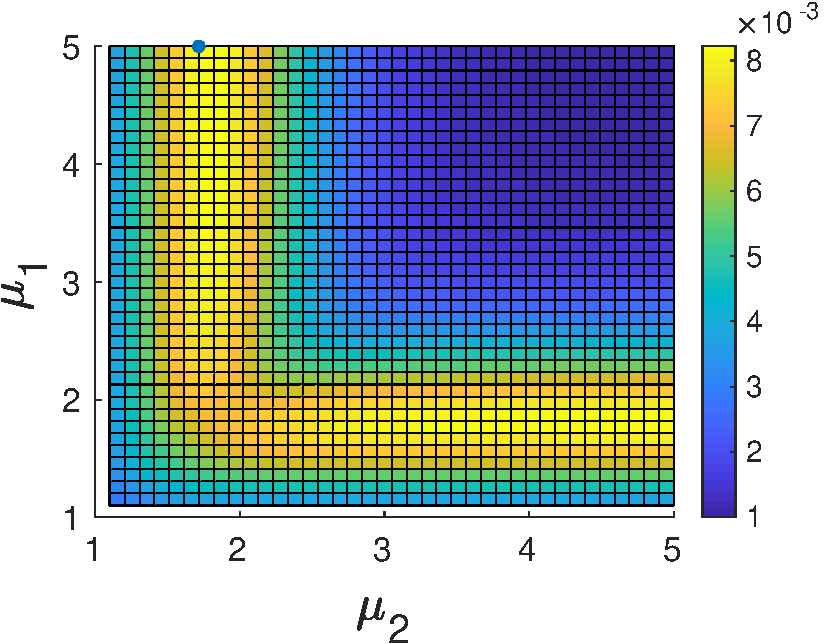
\includegraphics[width=.50\textwidth]{VisionSwitchingForager_J2_PowerLaw_ND_lambda1000_rv50-50}\label{fig:visionswitching_base}}\hfill
	\subfloat[{Switching between $r_v=50$ and $r_v=0$.}]{%
		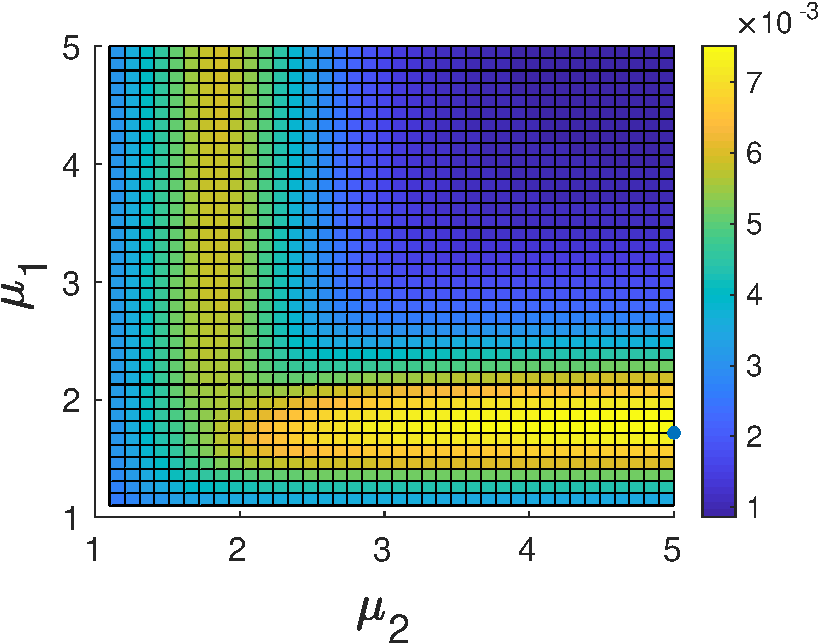
\includegraphics[width=.50\textwidth]{VisionSwitchingForager_J2_PowerLaw_ND_lambda1000_rv50-0}\label{fig:visionswitching_switch}}\\
	\caption[Efficiency of two-state Markov-modulated power-law strategy, with switching radius of vision]{The efficiency of a non-destructive search ($x_0=50$) where the forager switches between two power-law distributions with parameters $\mu_1$ and $\mu_2$, with equal probability of switching between states. The radius of vision is different for each subplot. The optimal efficiency is marked with a blue circle.}\label{fig:visionswitching}
\end{figure}
One important thing to note about \cref{fig:visionswitching_switch} is that the efficiency is not longer symmetric about the $\mu_1=\mu_2$ line, as it is for \cref{fig:visionswitching_base}. For both scenarios, large efficiencies occur for strategies that switch between a Brownian motion and a L\'{e}vy walk, though for the vision switching strategy the efficiency is much worse, as expected, if the Brownian motion occurs in state $1$ while the vision is low. 
\section{Optimal Markov-modulated search strategies for two-states, three states, and higher}
\label{sec:1dMMRW_all}
In \cref{sec:1dMMRW_GUT}, we used Markov-modulated random walk strategies to consider a giving-up time forager. These giving-up time strategies are a special case of Markov-modulated random walks in which there is an absorbing state. In this section, we consider more general Markov-modulated random walk strategies that do not necessarily have an absorbing state. For a strategy with two states, the Markov chain will have a transition matrix
\begin{equation}
\label{eq:1dresults:2state}
P = \begin{bmatrix}
1-a & a\\
b & 1-b
\end{bmatrix},
\end{equation}
where $a, b \in [0,1]$. For three states, the transition matrix is
\begin{equation*}
P = \begin{bmatrix}
1-a-b & a & b\\
c & 1-c -d & d\\
e & f & 1-e-f
\end{bmatrix},
\end{equation*}
where $a,b,c,d,e,f \in [0,1]$. 
We can continue in this manner, defining the transition matrix for higher-state Markov-modulated random walk strategies. 
A $J$-state Markov-modulated random walk will have $J^2-J$ free variables in its transition matrix.
For a $J$-state Markov-modulated random walk, we also have $J$ different step-length distributions. We choose these step-length distributions to all be unbounded power-law distributions, since they offered the highest efficiency in previous sections, although there is nothing preventing us from considering any other combination of distributions. Each step-length distribution may have a different parameter $\mu$, and we choose $\lmin = 1$ and $r_v=1$ for all distributions, for simplicity. Finally, the initial distribution of the Markov chain has $J-1$ parameters, since it must sum to one. Thus, we have $J$ different parameters for the distributions, $J^2-J$ for the transition matrix, and $J-1$ for the initial distribution, totalling $J^2+J-1$ parameters. The evaluation of the efficiency for any set of parameters also becomes slower for larger $J$, since the matrix $\Amat$ has dimensions $J(M-1)\times J(M-1)$. Because of this, we only consider search strategies with up to $J=3$ states.

We once again use Matlab's \emph{fmincon} to minimise the expected total travel length and hence maximise the efficiency. We begin with a strategy where $J=1$ with an initial guess of $\mu=2$. As we increase the number of states to $J$, we use the optimal solution for $J-1$ states to determine an initial guess for \emph{fmincon}. The transition matrix gets an extra column, with each element being $1/J$. To compensate and ensure the row sums equal $1$, the transition matrix elements from the previous solution are all scaled by $(J-1)/J$ so they sum to $1-(1/J)$ rather than $1$. We also add an extra row to the bottom of the previous transition matrix, with each element being $1/J$. For example, if the optimal solution for the $J=2$ strategy was given by \cref{eq:1dresults:2state}, then the initial guess for the $J=3$ strategy is
\begin{equation*}
P = \begin{bmatrix}
2(1-a)/3 & 2a/3 & 1/3\\
2b/3 & 2(1-b)/3 & 1/3\\
1/3 & 1/3 & 1/3
\end{bmatrix}.
\end{equation*}
Our initial guess for the new parameter $\mu$ is the mean of the other $\mu$ values. For the $J$ strategy, our initial guess for the initial distribution, we take the optimal choice for the $J-1$ strategy and add an element $1/J$ for the final state, and renormalise the other states by multiplying them by $(J-1)/J$. For example, if the $J=2$ had an optimal initial distribution of
\begin{equation*}
\vec{z_{0}} = (a,1-a),
\end{equation*}
with $a \in [0,1]$, then our initial guess for the initial distribution is
\begin{equation*}
\vec{z_0} = \left(2a/3, 2(1-a)/3, 1/3 \right).
\end{equation*}

\paragraph{Results of \emph{fmincon}}
For the $1$-state forager, the optimal strategy is $P=[1]$, $\vec{z_{0}}=[1]$, and $\mu = 1.8699$. This is a L\'{e}vy walk, matching the results we found in \cref{sec:1dMMRW_nonMM},

For the $2$-state forager, the optimal strategy is a transition matrix given by
\begin{equation*}
P = \begin{bmatrix}
0.9940  &  0.0060\\
0  &  1
\end{bmatrix},
\end{equation*}
an initial probability vector $\vec{z_{0}} = (1, 0)$ and distribution parameters $\vec{\mu} = (10,    1.5868)$. This result is interesting, since the optimal general $2$-state strategy is, in fact, a giving-up time strategy, with the same parameters as found in \cref{sec:1dMMRW_GUT}. This corresponds to a forager that begins using Brownian motion, before giving up after a geometrically distributed amount of time with an approximate mean of $166.66$ steps, before performing a L\'{e}vy flight with $\mu=1.5868$. 

For the $3$-state forager, the optimal strategy is a transition matrix given by
\begin{equation*}
P = \begin{bmatrix}
 0.9849  &  0 &   0.0151\\
0  &  1  &  0\\
0 &  0.0152   & 0.9848
\end{bmatrix},
\end{equation*}
an initial probability vector $\vec{z_{0}} = (1,0,0)$, and distribution parameters $\vec{\mu} = (10, 1.3908,    2.4368)$. This strategy once again corresponds to a giving-up time strategy that begins following a Brownian motion, before giving-up into a L\'{e}vy flight, with parameter $\mu = 2.4368$. Then, after some further time, the forager gives up again, and switches to a L\'{e}vy flight with $\mu = 1.3908$, which will somewhat resemble a ballistic path, due to the small $\mu$ parameter. The mean of both geometrically distributed giving-up time are approximately $66$ steps.